
The simplest non-degenerate distribution of connection probabilities
is a distribution that takes two values $x$, $y$ with probability $p$
and $1-p$ respectively. %
%
This distribution may be seen as a crude approximation to the
connection probabilities recently observed in visual cortex as a
function of the neurons’ difference of orientation preference
\cite{Lee2016}.
%
Formally, let $x,y \in [0,1]$ with $x > y$ and $0 < p
< 1$. A random variable $X$ follows the two-point distribution 
%%\cc{(\enquote{Zweitpunktverteilung},
%\href{https://de.wikipedia.org/wiki/Zweipunktverteilung}{Wiki})}
$\mathcal{T}(p,x,y)$ if $P(X=x)=p$ and $P(X=y) = 1-p$.
%

%
In our network model let then the $P_{ij}$ be $\mathcal{T}(p,x,y)$
distributed. The overall connection probability $\mu$ is
\begin{align}
\mu = \E(P_{ij}) = px + (1-p)y. \label{eq:bd1}
\end{align}
%% Given $\mu$,$x$ and $y$, the probability $p$ calculates as
%% \begin{align}
%%   p = \frac{c-y}{x-y}. \label{eq:bd1}
%% \end{align}
Assume again that $P_{ij} = P_{ji}$. The relative occurrence of
bidirectional connections is given by
\begin{align}
  \varrho = \frac{\E(P_{ij}^2)}{\mu^2} = \frac{p x^2 + (1-p) y^2}{\mu^2} \label{eq:bd2}
\end{align}
Solving \eqref{eq:bd1} for $p$ and inserting into
equation~\eqref{eq:bd2} yields an expression for the relative
overrepresentation depending on $x$, $y$ and $\mu$ (\cc{Appendix A1}),
\begin{align}
\varrho = \frac{x+y}{\mu} - \frac{xy}{\mu^2}.
\end{align}

\begin{figure}[h!]
\centering
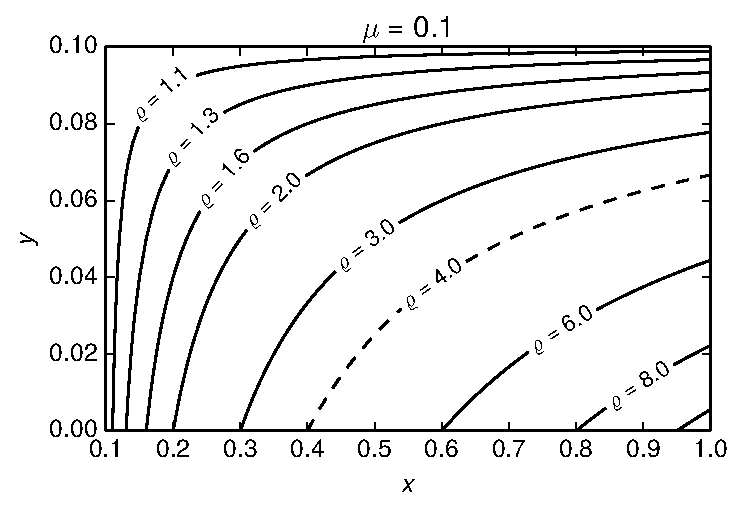
\includegraphics[width=0.675\textwidth]{%
  %../lab/two_point_distribution/contour_plot.pdf}
  img/contour_plot.pdf}
\caption{Contour plot shows the relative overrepresentation $\varrho$
  obtained from different pairings of $x$ and $y$ in a network with
  two-point distributed connection probabilities, $P_{ij} \sim
  \mathcal{T}(\frac{\mu-y}{x-y},x,y)$, and overall connection
  probability $\mu = 0.1$. The dashed line marks an overrepresentation
  of bidirectional connections of $\varrho=4$ as observed by
  \textcite{Song2005} in their experimental study.}
\label{fig:tp}
\end{figure}

In local cortical circuits, a single excitatory neuron is typically
projecting to roughly 10\% of the excitatory population.
%
Fixing $\mu = 0.1$, we obtain the relative occurrence dependent on the
two connection probability values $x$ and $y$.
%
Given $x \geq \mu$ it follows that $y \leq \mu$ (\cc{Appendix A2}) and
the possible values for $x$ and $y$ are $0.1 \leq x \leq 1$ and $0
\leq y \leq 0.1$.
%
Figure~\ref{fig:tp} shows contours of $\varrho$ for the $(x,y)$
pairings illustrating how different values for the relative
overrepresentation of reciprocal connections can be induced by
two-point distributed connection probabilities.
%
We find that in such networks higher values of $\varrho$ are easily
obtained with reasonable network configurations. %
%
For example, a relative overrepresentation of $\varrho=4$ could be
achieved by a two-point distribution of connection probabilities where
one group of neuron pairs is highly connected with probability
$x=0.7$, while the other group of neuron pairs is sparsely connected
with probability $y=0.05$.
%
The highly connected pairs then make up less than $8\%$ of all
neuronal pairs, showing that it is sufficient to have a small subgroup
of highly connected neuron pairs to induce a high overrepresentation
of bidirectionally connected pairs in the network.





